\chapter{Introduzione}

I due temi su cui verte la trattazione che segue mi appassionano particolarmente e, con questo documento, intendo prima analizzarli singolarmente e poi verificare l'esistenza di una eventuale relazione tra i due.

Il primo argomento è il riscaldamento globale. Da sempre, mi interesso dei temi ambientali e la mia quotidianità è spesso permeata da scelte che tengono in considerazione l'impatto e la sostenibilità delle mie azioni. Per questo, ispirato anche da una celebre frase di Greta Thunberg, \textit{"You are never too small to make a difference"}, illustrerò questo fenomeno e, più in particolare, l'impatto economico e sociale che sta avendo sulle nostre vite.

Altrettanto di attualità, il secondo tema è l'inflazione. In questi mesi, questa parola è stata spesso protagonista del dibattito pubblico e il principale motivo è che essa, così come il cambiamento climatico, ha effetti rilevanti sul nostro modo di vivere. Non solo, le dinamiche e le decisioni di politica monetaria, in questo periodo di incertezza e cambiamento, sono sempre più centrali e attese. Per questi motivi, si passerà in rassegna la definizione di inflazione e del mandato primario della Banca Centrale Europea.

A unire questi due temi sarà la presentazione delle conclusioni dello studio di Donata Faccia: \textit{"Feeling the heat: extreme temperatures and price stability"} \parencite{ECB:feeling_heat}. Principalmente, verrà proposta la parte quantitativa dell'articolo: dai dati utilizzati, ai risultati delle regressioni prodotte dagli autori.

Il fine ultimo di questa esposizione è enfatizzare l'importanza dei temi ambientali e climatici nelle decisioni di politica monetaria. L'ambiente può diventare un nuovo pilastro dei modelli decisionali, non solo perché influenza l'andamento dei prezzi, come si dimostrerà, ma anche, e soprattutto, gli equilibri sociali.

\mainmatter

\chapter{Definizioni}
\label{chp1}

\section{Il cambiamento climatico}
\label{chp1.1}

\begin{displayquote}
\small\singlespacing\textit{Climate change will amplify existing risks and create new risks for natural and human systems. Risks are unevenly distributed and are generally greater for disadvantaged people and communities in countries at all levels of development.} \parencite{IPCC:2014}
\end{displayquote}

Una delle maggiori sfide dei prossimi decenni sarà la mitigazione del cambiamento climatico. Negli ultimi trent'anni, questo fenomeno ha assunto rilevanza sempre maggiore, poiché è in grado di impattare negativamente sulla quotidianità delle persone, le attività produttive, gli ecosistemi e, in ultima istanza, sugli equilibri sociali e la sopravvivenza di qualsivoglia organismo vivente sul pianeta Terra.

Gran parte delle fondamenta scientifiche che muovono le politiche dei governi e delle istituzioni sovranazionali, così come l'opinione pubblica, sui temi ambientali, ma non solo, sono prodotte dall'\textit{Intergovernmental Panel on Climate Change} (IPCC). Costituita dalle Nazione Unite nel 1988, ai suoi lavori partecipano migliaia di scienziati provenienti da 195 Stati; è l'organizzazione internazionale che si occupa di valutare e produrre la letteratura scientifica sui temi del cambiamento climatico.

Come prima cosa è necessario chiarire che "riscaldamento globale" e "cambiamento climatico" non sono termini intercambiabili.

Con "riscaldamento globale", infatti, si identifica il continuo aumento delle temperature superficiali, causato dalla crescente concentrazione di gas serra, vedi Figura \ref{fig-ghg_concentration}, emessi dall'attività umana. I principali \textit{greenhouse gases} (GHG) rilasciati in atmosfera sono l'anidride carbonica ($\mathrm{CO_2}$), il metano ($\mathrm{CH_4}$) e l'ossido di diazoto ($\mathrm{N_2O}$). Questi gas hanno la capacità di trattenere parte delle radiazioni solari che colpiscono la Terra, provocando di conseguenza l'aumento delle temperature superficiali. Malgrado la crescente diffusione di politiche indirizzate a ridurre la produzione di gas serra, la loro concentrazione nell'atmosfera è comunque aumentata e la crescita economica e demografica mondiale ne sono le principali cause in assoluto \parencite{IPCC:2014}.

\begin{figure}
	\centering
	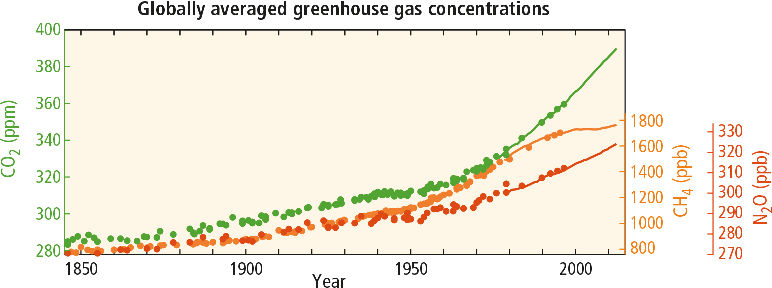
\includegraphics[width=0.80\textwidth]{img/ghg_concentration.pdf}
	\caption{}
	\source{\cite{IPCC:img:ghg_concentration}}
	\label{fig-ghg_concentration}
\end{figure}

"Cambiamento climatico" riassume i crescenti e persistenti mutamenti, in media e o nella variabilità, di diversi indicatori climatici, ad esempio di precipitazione, vento o temperatura. Nella storia della Terra, i cambiamenti climatici si sono sempre verificati. Ciò che sta avvenendo negli ultimi anni però, non è solo un processo naturale, perché ad esso si sono sommati gli effetti causati dall'uomo \parencite{IPCC:2014}.

Questi fenomeni lasciano intuire futuri scenari che solo in parte posso essere previsti e le cui conseguenze non possono far altro che alterare il modo in cui ora siamo abituati a vivere. Per esempio, già in Italia, come in molte altre regioni del Pianeta, i cambiamenti legati alla frequenza e all'intensità delle precipitazioni e il progressivo scioglimento delle riserve idriche dei ghiacciai, stanno complicando il reperimento dell'acqua necessaria per le attività agricole, con chiari impatti anche sulla sicurezza alimentare. Il surriscaldamento delle temperature può scatenare, e già lo sta facendo, conseguenze travolgenti: l'estinzione di specie animali, complicanze sulla salute delle persone e in particolare nei paesi in via di sviluppo, migrazioni di massa \parencite{IPCC:2014}.

In conclusione, gli effetti già visibili del cambiamento climatico e le previsioni di quelli futuri richiedono un intervento sempre più immediato degli Stati e delle comunità internazionali. Ognuno di noi deve quindi sentirsi coinvolto e nella sua quotidianità attivarsi in azioni che possano alleggerire la nostra impronta climatica. Il progresso tecnologico giocherà senz'altro un ruolo cruciale nei prossimi anni, soprattutto per garantire fonti energetiche più pulite. Le motivazioni che possono spingerci ad attivarci per il Pianeta sono diverse: la conservazione degli ecosistemi, la protezione della nostra specie e delle altre, oppure, la solidarietà e il sostegno ai Paesi in via di sviluppo, che inevitabilmente nei prossimi anni dovranno affrontare sfide complicate. E forse, un nostro intervento oggi potrà alleggerire la loro, ma anche la nostra, minaccia dietro l'angolo.

\section{L'inflazione}

I prezzi di beni e servizi cambiano continuamente. La loro variazione muta il potere d'acquisto della moneta che gli individui possiedono e spendono quotidianamente. Un aumento generalizzato dei prezzi prende il nome di inflazione, mentre una riduzione si chiama deflazione \parencite{ECB:inflation_def}.

Gli indici dei prezzi al consumo fanno parte delle statistiche ufficiali di contabilità nazionale e sono i principali strumenti a cui si fa ricorso per la rilevazione dell'inflazione. In Italia, l'ISTAT produce tre indici: il NIC, per l'inflazione dell'intero sistema economico italiano; il FOI, che si riferisce ai consumi di una famiglia con a capo un lavoratore dipendente; e l'IPCA (o HICP \textit{Harmonised Index of Consumer Prices}), ottenuto secondo le metodologie Eurostat. Gli istituti di statistica nazionale sono incaricati della costruzione degli indici e del loro aggiornamento, monitorando le abitudini di spesa dei consumatori nazionali e della rilevazione dei prezzi. Questi indici registrano periodicamente i prezzi di un paniere rappresentativo di beni e servizi acquistati dai consumatori.  Il rapporto con il periodo di riferimento permette di calcolarne il tasso di variazione \parencite{ISTAT:indici}.

\begin{figure}[h]
	\centering
	\includegraphics[width=0.80\textwidth]{img/istat_pesi_paniere_2002_2022.pdf}
	\caption{}
	\source{elaborazione su dati \cite{ISTAT:pesi_paniere_2022}}
	\label{img:istat_pesi_paniere_2002_2022}
\end{figure}

In Europa, l'indice ufficiale per la misurazione dell'inflazione è l'HICP. \'E un indice le cui categorie di beni e servizi sono stabilite dall'\textit{European Classification of Individual Consumption by Purpose} (ECOICOP). Per questo, si dice avere un paniere costante (\textit{fixed-basket}), anche se i beni contenuti nelle diverse categorie e il peso delle stesse, viene aggiornato annualmente \parencite{ECB:measuring_inflation}. La Figura \ref{img:istat_pesi_paniere_2002_2022} mostra come, nel periodo 2002-2022, siano cambiati i pesi delle diverse categorie del paniere.

Esistono diverse formule su cui basare il calcolo di un indice e le principali sono dovute agli studi di Fisher, Paasche o Laspeyres, quest'ultima utilizzata dall'HICP.

\begin{equation}
	P = \sum{\frac{p^t}{p^0} \cdot w^{0}}
\end{equation}

Dove $P$ è il valore dell'indice, $p^0$ è il prezzo della categoria al tempo base e $p^t$ è il suo prezzo al tempo successivo. $w^0$ è il peso della categoria nell'indice, ossia la sua  rilevanza in proporzione alla spesa complessiva del Paese \parencite{Eurostat:layeres_formula}.

\begin{figure}[h]
	\centering
	\includegraphics[width=0.80\textwidth]{img/inflation_1990_2020.pdf}
	\caption{}
	\source{elaborazione su dati \cite{WB:img:inflation_1990_2020}}
	\label{img:inflation_1990_2020}
\end{figure}

La Figura \ref{img:inflation_1990_2020} mostra l'andamento dell'inflazione, in termini di prezzi al consumo, dal 1960 al 2020 in cinque diversi Stati. Si può notare come, nei diversi Paesi, l'inflazione segua tendenzialmente un canale comune. \'E ben visibile l'effetto sull'inflazione delle crisi energetiche del 1973 e 1979 dovuto inizialmente al prezzo del petrolio imposto dal cartello dell'OPEC (\textit{Organization of the Petroleum Exporting Countries}) e, in seguito, causato dalle interruzioni della produzione del greggio durante la rivoluzione iraniana, periodo durante il quale il prezzo dell'energia aumentò vertiginosamente. Il costo maggiore dell'energia trainò l'aumento dei prezzi di beni e servizi. Al contrario, alla crisi finanziaria del 2008 seguì una grave recessione che ridusse la domanda di beni e servizi. I prezzi al consumo crollarono, portando l'inflazione anche in territorio negativo. Tornando ai giorni nostri, i \textit{lockdown} imposti, durante il corso del 2020, hanno impedito il normale svolgimento di numerose attività produttive e hanno portato al crollo del prezzo dell'energia. Dal lato della domanda si sono visti effetti discordanti tra loro: nei settori più colpiti dalle restrizioni, la domanda si è azzerata, mentre in altri, come l'alimentare o il tecnologico, si è verificato un aumento dei prezzi. La commistione di questi effetti ha portato nel corso del 2020 a una ritrovata deflazione \parencite{Blanchard_macroeconomia}. Oggi, nei primi mesi del 2022, a causa delle forti tensioni geopolitiche derivanti dal conflitto russo-ucraino e da un'economia surriscaldata, il mondo intero, in particolare l'Europa, sta sperimentando una fase inflazionistica. La Figura \ref{img:inflation_ea_2022} mostra la variazione mensile e percentuale dell'indice armonizzato dei prezzi al consumo nell'area Euro.

\begin{figure}[h]
	\centering
	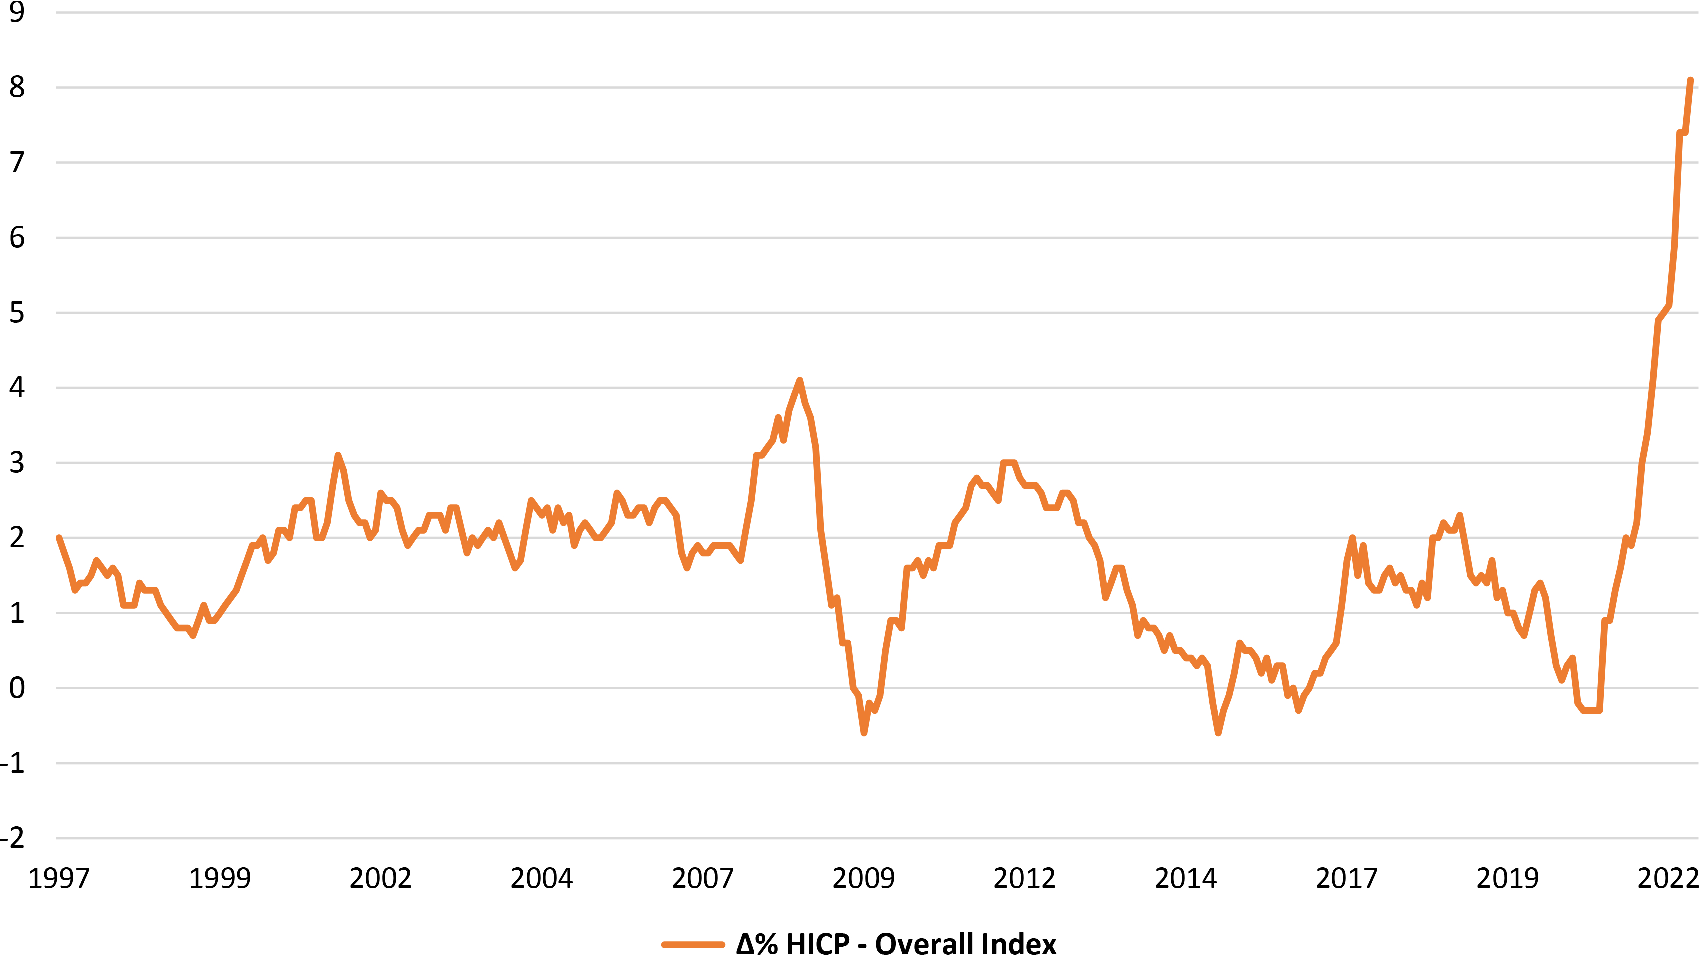
\includegraphics[width=0.80\textwidth]{img/inflation_ea_2022.pdf}
	\caption{}
	\source{elaborazione su dati \cite{ECB:ea_inflation_2022}}
	\label{img:inflation_ea_2022}
\end{figure}

Ma non sono solo gli shock, per definizione imprevisti e temporanei, a causare la costante fluttuazione dei prezzi. Esistono infatti, diverse teorie economiche e scuole di pensiero, in disaccordo tra loro, che cercano di spiegare le cause che determinano l'inflazione, in particolare di lungo periodo. La prima è quella sostenuta dai keynesiani, tra i quali si annovera Robert J. Gordon. Essi sostengono l'importanza della politica fiscale e i movimenti di domanda e offerta quali principali determinanti dei prezzi. Se questa visione può avere qualche riscontro empirico nel breve e medio termine, la tesi più largamente accettata, in particolare per spiegare l'inflazione di lungo periodo, è quella dei monetaristi \parencite{Blanchard_macroeconomia}. Milton Friedman scriveva: \textit{"The central fact is that inflation is always and everywhere a monetary phenomenon. Historically, substantial changes in prices have always occurred together with substantial changes in the quantity of money relative to output"} \parencite{Friedman_monetarism}. Questa affermazione trova pieno riscontro empirico nel grafico della Figura \ref{img:inflation_m2}, dove si mettono a confronto le variazioni percentuali dei prezzi al consumo con quelle dell'aggregato monetario M2, entrambe con frequenza mensile e riguardanti l'area Euro. La differenza temporale tra il movimento dell'offerta di moneta e quello dell'inflazione è determinato dalla velocità di circolazione del denaro nell'economia.

\begin{figure}[h]
	\centering
	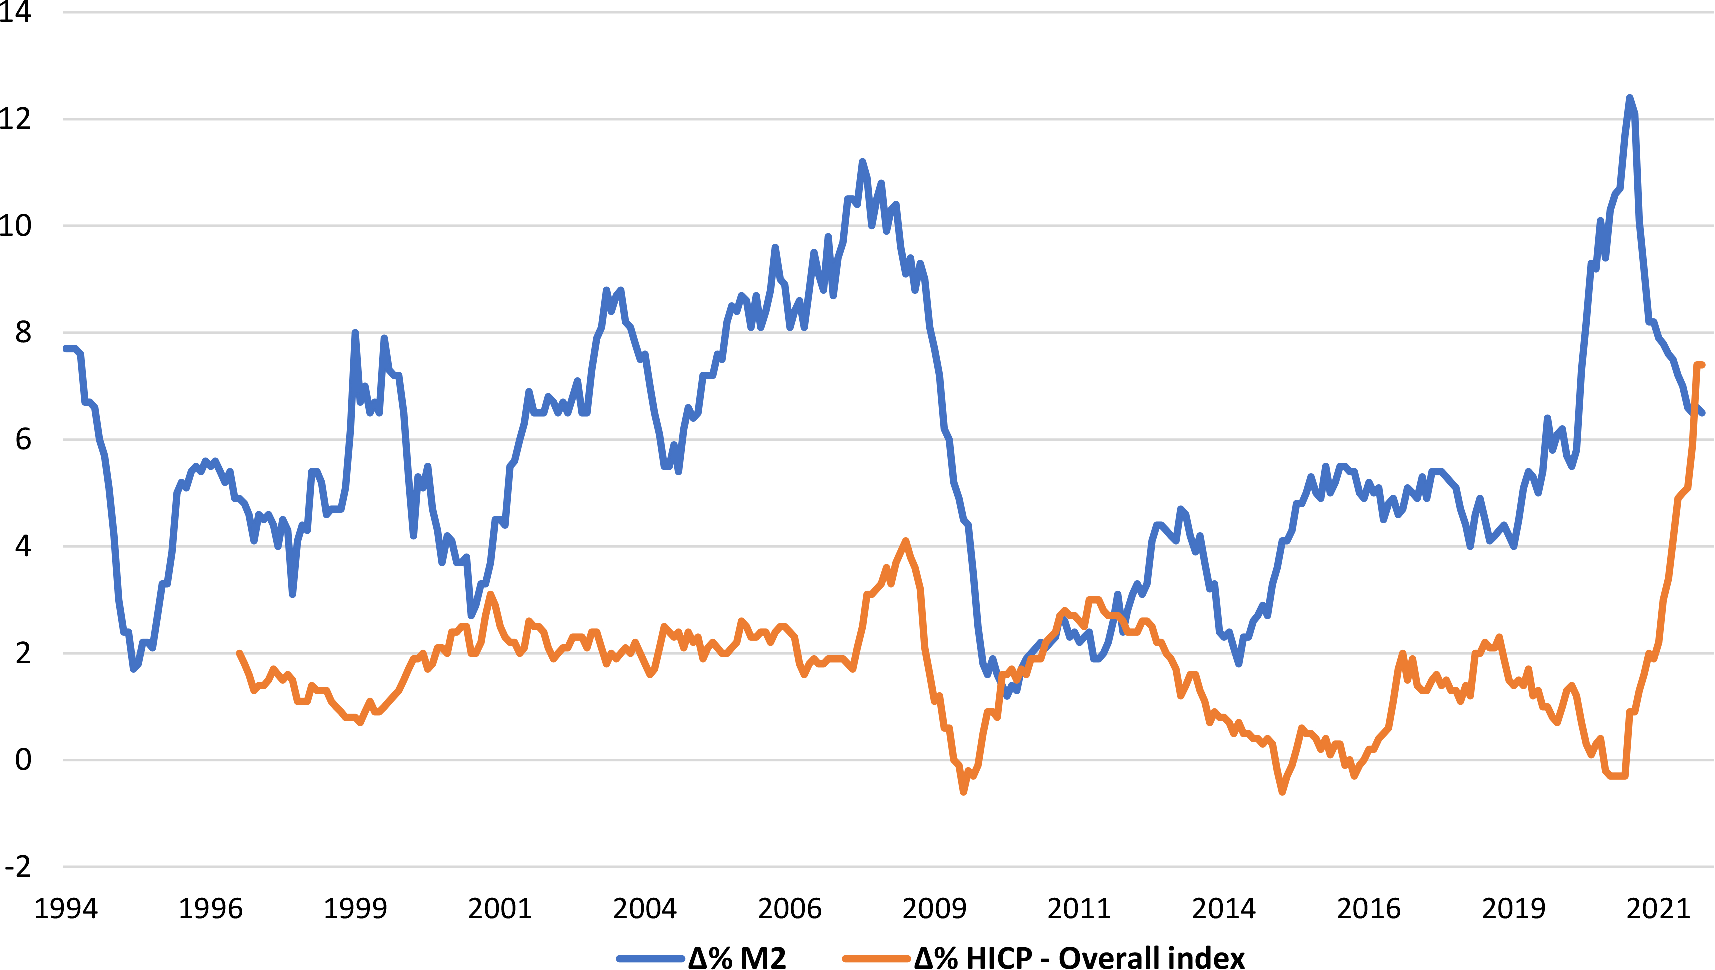
\includegraphics[width=0.80\textwidth]{img/inflation_m2.pdf}
	\caption{}
	\source{elaborazione su dati \cite{ECB:ea_inflation_2022}}
	\label{img:inflation_m2}
\end{figure}

Il motivo per cui consumatori, imprese e governi sono sensibili e influenzati dalle variazioni del tasso di inflazione è l'inesistenza di un'esclusiva \textit{pure} o \textit{core} \textit{inflation}. David Hume la interpretò così: "\textit{Imagine that all prices increase in the same proportion, but no relative price changes}". \'E inflazione pura o \textit{core} la componente della variazione di prezzo, equi-proporzionale e comune a tutti i prezzi. Se l'aumento generalizzato dei prezzi fosse per intero causato da un'inflazione pura e fosse seguito da un aumento dei salari nominali, le scelte degli agenti economici non muterebbero, perché i prezzi relativi non varierebbero. La variazione dei prezzi relativi rappresenta un primo costo dell'inflazione, seguita da una crescente incertezza nelle decisioni di spesa e allocazione delle risorse. Si è meno propensi a stipulare contratti di lungo termine, perché si è incerti sull'inflazione futura e quindi sui suoi effetti. Ancora più rilevante, soprattutto in presenza di un'inflazione non anticipata e salari non indicizzati, è l'effetto sulla distribuzione del reddito che assottiglia il salario reale dei lavoratori.
	
\begin{equation}
	\label{formula:salario_nominale}
	W = P\cdot F(u,z)
\end{equation}

\begin{equation}
	\label{formula:salario_reale}
	\frac{W}{P} = F(u,z)
\end{equation}

Nell'Equazione \ref{formula:salario_nominale}, $W$ è il salario nominale, $P$ è il livello dei prezzi, $F$ è una funzione definita dal livello di disoccupazione $u$ e da $z$ che raggruppa tutte le altre variabili che influenzano la determinazione del salario. L'Equazione \ref{formula:salario_reale} mostra il salario reale. All'aumentare del livello dei prezzi, il salario reale si riduce. Infine, i lavoratori possono essere ulteriormente colpiti dal drenaggio fiscale o \textit{fiscal drag}. In presenza di salari adeguati automaticamente all'inflazione, ma scaglioni di imposta non mobili, i lavoratori possono vedersi aumentata la pressione fiscale sul loro salario reale. All'aumentare di $P$, con l'adeguamento salariale aumenta anche il salario lordo nominale $W$. Se al lavoratore viene applicata l'imposizione maggiore di uno scaglione superiore, in realtà, il suo salario netto reale sarà minore \parencite{Blanchard_macroeconomia}.

Questi ultimi paragrafi mostrano la rilevanza che l'inflazione assume quale indicatore dell'andamento di un'economia. Un aumento incontrollato dei prezzi può avere gravi conseguenze sui mercati e sulla vita delle persone e per questo deve essere gestito. Oltre alle cause già illustrate in questo Capitolo \ref{chp1}, nelle pagine successive si illustrerà l'effetto che anche i cambiamenti climatici, e in particolare il riscaldamento globale, hanno sui prezzi.